\documentclass[12pt]{kiarticle} % You can learn about my document class "kiarticle" and install it to your device by following the link: https://github.com/Kiarendil/toolkitex
\graphicspath{{pic/}}
\DeclareGraphicsExtensions{.pdf,.png,.jpg,.eps}
%%%
\pagestyle{fancy}
\fancyhf{}
%\renewcommand{\headrulewidth}{ 0.1mm }
\renewcommand{\footrulewidth}{ .0em }
\fancyfoot[C]{\texttt{\textemdash~\thepage~\textemdash}}
\fancyhead[L]{Пинч-эффект \hfil}

\usepackage{multirow} % Слияние строк в таблице
\newcommand
{\un}[1]
{\ensuremath{\text{#1}}}
\newcommand{\eds}{\ensuremath{ \mathscr{E}}}


\begin{document}
	
	\begin{titlepage}
		\begin{center}
			\large 	Московский физико-технический университет \\
			Факультет иноваций и высоких технологий \\
			\vspace{0.2cm}
			
			\vspace{4.5cm}
			Вопрос по выбору на тему: \\ \vspace{0.2cm}
			\LARGE \textbf{Пинч-эффект в плазме}
		\end{center}
		\vspace{2.3cm} \large
		
		\begin{center}
			Работу выполнила: \\


			\vspace{10mm}
			
			
			
			
		\end{center}
		
		\begin{center} \vspace{60mm}
			г. Долгопрудный \\
			2020 год
		\end{center}
	\end{titlepage}
	
	
	\section{Введение}
	Плазму можно создать с помощью электрического разряда. Далее возникает задача удержать образовавшийся плазменный шнур от рысплывания, обусловленного существующим в нём газокинетическим давлением. Этой цели можно добиться, используя различные приёмы, к числу которых относится пинч эффект.
	\par \textbf{Пинч-эффект} (англ. pinch - сужение, сжатие) --- эффект сжатия токового канала под действием магнитного поля, индуцированного самим током. Сильный ток, протекающий в плазме, твёрдом или жидком металле создаёт магнитное поле. Оно действует на заряженные частицы (электроны и/или ионы), что может сильно изменить распределение тока. При больших токах сила Ампера приводит к деформации проводящего канала, вплоть до разрушения. В природе наблюдается в молниях.
	\par Различают два основных типа пинч-эффекта:
	\begin{itemize}
		\item z-пинч --- ток течет вдоль плазменного шнура и взаимодействует с собственным магнитным полем;
		\item $\Theta$-пинч --- на плазменный шнур накладывается продольное магнитное поле, создающее кольцевые токи в результате взаимодействия которых с полем происходит сжатие шнура.
	\end{itemize}
	
	\begin{figure}[h]
		\begin{center}
			\begin{minipage}[h]{0.4\linewidth}
				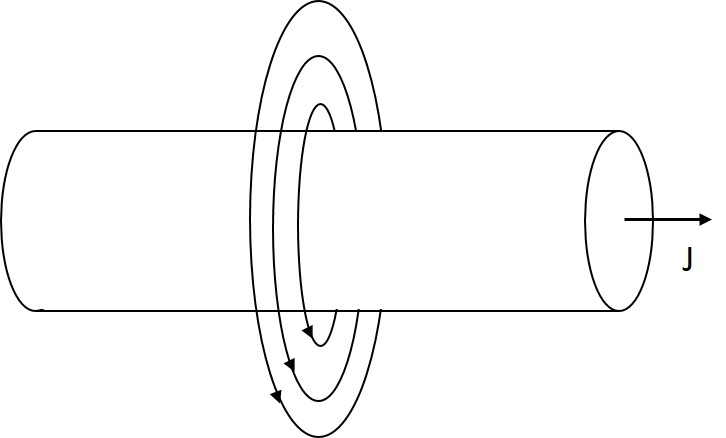
\includegraphics[width=1\linewidth]{Pic1.jpg}
				\caption{z-пинч} %% подпись к рисунку
				\label{pic1a} %% метка рисунка для ссылки на него
			\end{minipage}
			\hfill
			\begin{minipage}[h]{0.4\linewidth}
				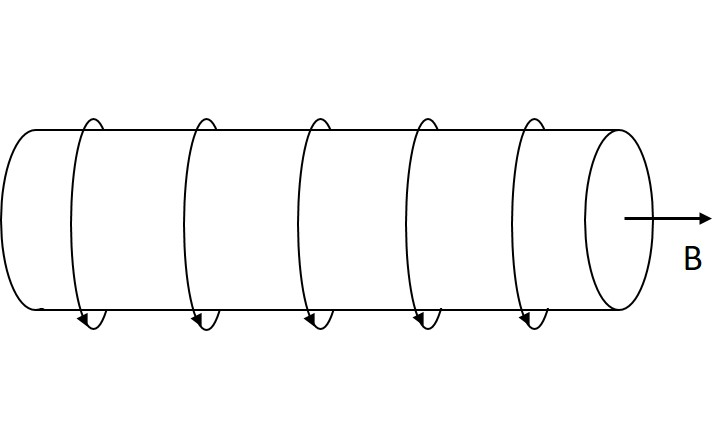
\includegraphics[width=1\linewidth]{Pic2.jpg}
				\caption{$\Theta$-пинч}
				\label{pic1b}
			\end{minipage}
		\end{center}
	\end{figure}
	\section{Равновесие z-пинча}
	Рассмотрим подробнее z-пинч. Будем считать, что:
	\begin{enumerate}
		\item Плотность тока постоянна по сечению плазменного шнура: $j(\textbf{r}) = const$, так что полный ток $J = jS = \pi R^2 j$;
		\item Концентрация частиц постоянна: n(\textbf{r}) = const
	\end{enumerate}
	Магнитное поле внутри шнура находится с помощью теоремы о циркуляции магнитного поля:
	\[ \oint {\textbf{H} d\textbf{l}} = 2 \pi r H = \dfrac{4\pi}{c} J(r) = \dfrac{4\pi}{c}j \cdot \pi r^2.  \]
	Отсюда находим:
	\[ j = \dfrac{c}{2 \pi r}B.  \]
	Согласно основному уравнению магнитной гидродинамики условие равновесия плазмы можно записать в виде:
	\[ \mathrm{grad} P = \dfrac{1}{c}[\textbf{j} \times \textbf{B}]  \]
	\begin{wrapfigure}[22]{r}{0.3\linewidth} 
	
		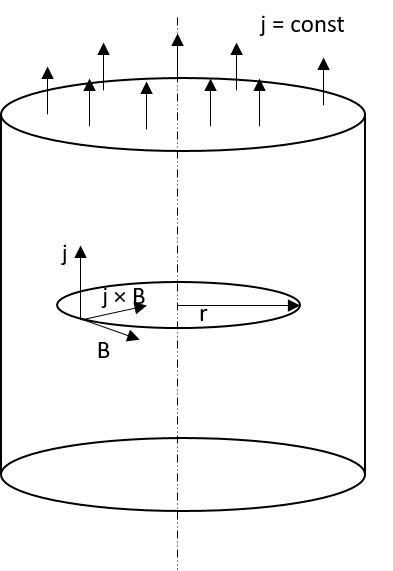
\includegraphics[width=\linewidth]{Pic3.png}
		\caption{К выводу условия равновесия z-пинча.}
		\label{Pic3}
	\end{wrapfigure}
	Поскольку $j \perp B$, то, как видно из рисунка \ref{Pic3} вектор $\textbf{j} \times \textbf{B}$ направлен к оси цилиндра, причем:
	\[ (j \times B)_к = -jB = -\dfrac{2\pi}{c} j^2r   \]
	Соответственно условие равновесия принимает вид:
	\[ \dfrac{dP}{dr} = -\dfrac{2\pi}{c^2}j^2r \ \ \Rightarrow \ \ P + \dfrac{\pi}{c^2}j^2r^2 = const \]
	Заменяя в этом равенстве
	\[  P = nkT, \ \ j = \dfrac{c}{2\pi r}B, \]
	перепишем условие равновесия следующим образом:
	\[ nkT(r) + \dfrac{B^2(r)}{4\pi} = const  \]
	Полученное равенство можно интерпретировать таким образом, что сумма газокинетического ($nkT$) и магнитного $(\dfrac{B^2}{4\pi})$ давлений должна быть постоянной в объёме плазмы.
	\par Полагая на внешней границе плазменного шнура $T(R) = 0$ получаем:
	\[ T(r) = \dfrac{1}{4\pi kn}\left[ B^2(R) - B^2(r) \right].  \]
	Этому соотношению можно придать другой вид, воспользовавшись формулой
	\[  B = \dfrac{2\pi}{c}jr = \dfrac{2J}{cR^2}r. \]
	Это даёт 
	\[ T(r) = \dfrac{\pi}{nc^2}\left( \dfrac{J}{\pi R^2} \right)^2(R^2 - r^2).  \]
	В частности, отсюда следует
	\[ N_1kT(0) = \dfrac{J^2}{c^2},  \]
	где введена погонная плотность частиц плазменного шнура на его оси $N_1 = \pi R^2 n$.
	\par Полученное равенство называется \textbf{условием равновесия Беннета}.
	\section{Неустойчивость z-пинча}
	Плазма - это объект, в котором наблюдаются различные неустойчивости, приводящие к нарушению её однородности, формы. Неустойчивости в свою очередь ограничивают время жизни плазмы. Данное обстоятельство оказывается особенно критичным в задачах термоядерного синтеза, когда плазму требуется удерживать длительное время, чтобы активировать реакцию.
		\begin{wrapfigure}[11]{r}{0.5\linewidth} 
		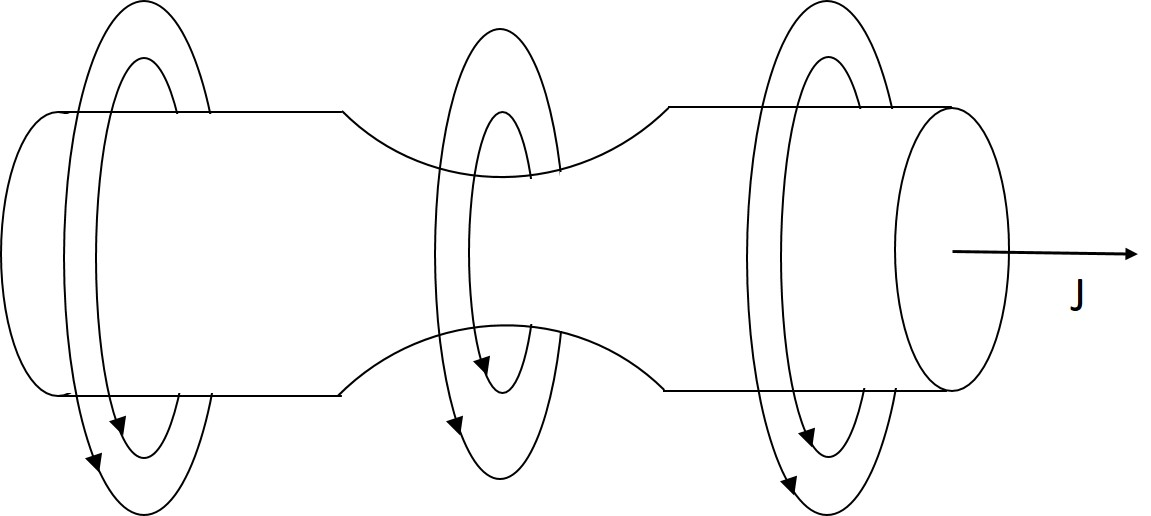
\includegraphics[width=\linewidth]{Pic4.jpg}
		\caption{Неустойчивость z-пинча --- возникновение перетяжек плазменного шнура}
		\label{Pic4}
	\end{wrapfigure}
	\par К числу неустойчивостей пинча относится возникновение и развитие перетяжек, как это проиллюстрировано на рисунке \ref{Pic4}. Рассмотрим данное явление на примере z-пинча. Механизм возникновения перетяжек можно пояснить следующим образом. Пусть в каком-то месте шнура случайным образом возникло сужение. Поскольку ток, текущий по шнуру, постоянный, то плотность тока возрастает по закону $j = J/ \pi R^2$. На поверхности шнура действует магнитное поле $B(R) = 2J/cR$. В результате возрастает амперова сила, сжимающая шнур:
	\[  F_A = \dfrac{1}{c}jB(R) = \dfrac{1}{c} \dfrac{J}{\pi R^2} \dfrac{2J}{cR} = \dfrac{2J^2}{c^2\pi R^3}.  \]
	Отсюда следует, что сжимающее действие магнитного поля не уравновешивается газокинетическим давлением $P$, практически не меняющимся в этом месте. В итоге происходит дальнейшее сужение перетяжки --- развивается неустойчивость.
	\par Для борьбы с данной неустойчивостью было предложено "вморозить" в плазму продольное магнитное поле $B_z^{(e)}$. Поскольку магнитный поток в проводящей среде сохраняется:
	\[ \Phi = \pi R^2 B_z^{(e)} = const,  \]
	то при сужении шнура поле возрастает:
	\[ B_z^{(e)} \sim 1/R^2.  \]
	Вклад этого поля в плотность энергии $\varDelta U \sim B_z^{(e)2} \sim 1/R^4.$ Считаем систему замкнутой, так что работа поля осуществляется за счёт его энергии:
	\[ \delta A_{поле} = f\delta R = -\delta U \sim \delta R/R^5 \]
	Следовательно, $f \sim 1/R^5 > 0$, то есть возникающая сила противодействует сжимающей пучок амперовой силе. Кроме того, при уменьшении радиуса пучка эта сила по величине растёт быстрее, чем амперова сила $(F_A \sim 1/R^3)$. Таким способом можно стабилизировать z-пинч.
	\section{Основное уравнение магнитной гидродинамики плазмы}
	Выделим в плазме элемент объема $dV = dxdydz$. Обозначим газокинетическое давление, действующее в плазме как $P(x,y,z)$. Тогда вдоль оси $x$ на элемент объёма будет действовать сила
	\begin{wrapfigure}[10]{r}{0.4\linewidth} 
		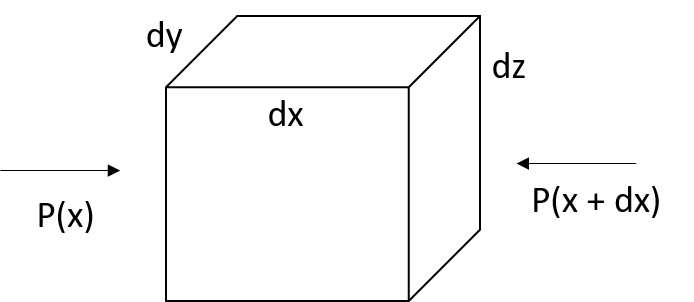
\includegraphics[width=\linewidth]{Pic5.png}
		\caption{К расчету сил, действующих на элемент объёма плазмы благодаря газокинетическому давлению.}
		\label{Pic4}
	\end{wrapfigure}
	\[  df_x = [P(x,y,z) - P(x+dx, y,z)] dydz = -\dfrac{\partial P}{\partial x}dV.  \]
	Аналогично вдоль осей $y$ и $z$ будут действовать силы
	\[ df_y = -\dfrac{\partial P}{\partial y}dV, \ \ df_z = -\dfrac{\partial P}{\partial z}dV.  \]
	В векторном виде сила записывается в виде $d\textbf{f} = -gradP\x dV$.
	\par Запишем уравнение движения рассматриваемого элемента объёма. Пусть $\rho_M$ - массовая плотность плазмы, так что масса элемента объёма равна $dm = \rho_M dV$. Тогда согласно второму закону Ньютона имеем
	\[ dm \dfrac{d\textbf{v}}{dt} = - \mathrm{grad} P \x dV, \ или \ \ \rho_M \dfrac{d\textbf{v}}{dt}= -\mathrm{grad} P. \]
	Полученное уравнение определяет поведение плазмы в отсутствие каких-либо иных сил, кроме газокинетического давления.
	\par Поскольку в плазме движутся заряды, то они создают токи, которые приводят к появлению магнитных полей. Эти поля в свою очередь создают силы Ампера, действующие на токи.
	\par Сила Ампера, действующая на элемент объема $dV$, в котором присутствует ток с плотностью $j$, равна
	\[  d\textbf{F}=\dfrac{1}{c} \textbf{j} \times \textbf{B} dV. \]
	С учётом этого уравнения движения принимает вид
	\[  \rho_M \dfrac{d\textbf{v}}{dt}= -\mathrm{grad} P + \dfrac{1}{c} \textbf{j} \times \textbf{B}. \]
	
\end{document}